\documentclass[11pt, oneside]{article}   	% use "amsart" instead of "article" for AMSLaTeX format
\usepackage{geometry}                		% See geometry.pdf to learn the layout options. There are lots.
\geometry{letterpaper}                   		% ... or a4paper or a5paper or ... 
%\geometry{landscape}                		% Activate for for rotated page geometry
%\usepackage[parfill]{parskip}    		% Activate to begin paragraphs with an empty line rather than an indent
\usepackage{graphicx}				% Use pdf, png, jpg, or eps§ with pdflatex; use eps in DVI mode
								% TeX will automatically convert eps --> pdf in pdflatex		
\usepackage{amsmath, amssymb}    % May not all be necessary
\usepackage{graphicx}                    % For including pictures
\usepackage{hyperref}                    % For formatting (clickable) URLs
\usepackage{algpseudocode}
\usepackage{algorithm}
\usepackage{mfirstuc}
\usepackage{graphicx}
\usepackage{amsopn}
\usepackage{url}
\usepackage{parskip}
\usepackage{wrapfig}
\usepackage{color}
\usepackage[usenames,dvipsnames,svgnames,table]{xcolor}
\usepackage{grffile}
\usepackage{comment}
\usepackage{epsfig}
\usepackage{float}
\usepackage{subfigure}
\usepackage{verbatim}
\usepackage{multirow}
\usepackage{todonotes}
\usepackage{epstopdf}
\usepackage{amssymb}
\usepackage{multirow}
\usepackage{hhline}

\presetkeys{todonotes}{inline}{}

\newcommand\figref{Fig.~\ref}
\newcommand\secref{Section~\ref}
\newcommand\tabref{Table~\ref}

\title{CS 659 Course Project \\ Restaurant Revenue Prediction}
\author{Huangxin Wang and Zhonghua Xi \\
\\
Computer Science Dept. \\
George Mason University}
%\date{}							% Activate to display a given date or no date

\begin{document}
\maketitle

\section{Introduction}
\todo{re-phrase this section}
Deciding when and where to open new restaurants is largely a subjective process based on the personal judgement and experience of development teams. 
This subjective data is difficult to accurately extrapolate across geographies and cultures.
New restaurant sites take large investments of time and capital to get up and running. 
When the wrong location for a restaurant brand is chosen, the site closes within 18 months and operating losses are incurred. 
Finding a mathematical model to increase the effectiveness of investments in new restaurant sites would allow funds to invest more in other important business areas, like sustainability, innovation, and training for new employees.
The goal of this project is to predict the revenues of restaurants by given demographic, real estate, and commercial data of existing restaurants withe their current revenues.

%\subsection{}
\section{Dataset}
We collect the data from Kaggle, a community of data scientists which also hosts data science competitions. 
Restaurant revenue prediction is one of the active competition.
There are 137 restaurants in the training set and 100000 in the test set which is an unbalanced dataset. 
For each record, 41 features are given detailed in \tabref{tab:features}.

\begin{table}[htdp]
\footnotesize
\caption{Features}
\begin{center}
\begin{tabular}{|r|l|}
\hline
\bf{Name} 		& \bf{Description} \\ \hline
\bf{Open Date}	& Categorical. Opening date for a restaurant. \\ \hline
\bf{City}		& Categorical. City that the restaurant is in. \\ \hline
\bf{City Group} & Categorical. Type of the city. Big cities, or Other. \\ \hline
\bf{Type}		& \begin{tabular}{@{}l@{}} Categorical. Type of the restaurant. \\ FC: Food Court, IL: Inline, DT: Drive Thru, MB: Mobile. \end{tabular}   \\ \hline
\bf{P1-P37}		& \begin{tabular}{@{}l@{}} Numerical. Three categories of these obfuscated data. \\ 
\bf{Demographic data} \\
Gathered from third party providers with GIS systems. \\ 
These include population in any given area, age and \\
gender distribution, development scales. \\
\bf{Real estate data} \\
Mainly relate to the m2 of the location, front facade \\
of the location, car park availability. \\
\bf{Commercial data} \\
Mainly include the existence of points of interest \\
including schools, banks, other QSR operators. \end{tabular}   \\ \hline
\bf{Revenue}	& \begin{tabular}{@{}l@{}} A transformed revenue of the restaurant in a given year \\
Only provided in training set.
\end{tabular} \\ \hline
\end{tabular}
\end{center}
\label{tab:features}
\end{table}%

\subsection{Evaluation}
\subsubsection{What to submit?}
For each records in the test set, output the ID of that record followed by the predicted revenue.

\subsubsection{Evaluation Metric}
Submissions are scored on the root mean squared error. 
RMSE is very common and is a suitable general-purpose error metric. 
Compared to the Mean Absolute Error, RMSE punishes large errors:
\begin{equation*}
RMSE = \sqrt{\frac{1}{n} \sum_{i=1}^{n} (y_i - \hat{y}_i)^2 }, 
\end{equation*}
where $\hat{y}_i$ is the predicted revenue and $y_i$ is the ground truth.

\subsubsection{Public Board V.S. Private Board}
For an active competition, each submission will be evaluated only on the 30\% of test set and scores will be published on the public board.
Once the competition is over, the final score is evaluated on the rest 70\% of the test set which will be published on the private board. 
Who win the public board may not win the private board since his model may be overfitted the public board's test data.
   
\subsection{Data Preparation}
\subsubsection{Revenue at a Glance}
In \figref{fig:revenue} we show the histogram of the revenues in the training set, from which we can see that majority of the revenues are around $5 \times 10^6$, 
however, there are few ``outliers'' which makes both training and prediction hard especially under RMSE evaluation metric.

\begin{figure}[htbp] %  figure placement: here, top, bottom, or page
   \centering
   \includegraphics[width=5in]{figs/revenue.eps} 
   \caption{Histogram of revenues.}
   \label{fig:revenue}
\end{figure}

\subsubsection{Features Selection}

{\bf Missing Categories} 
After a quick exploration of both training set and test set we found that both {\bf City} and {\bf Type} features have unseen categories in the training set.
There are total 63 cities in the entire dataset, too many new features will be added if we create a binary feature for each city and 
the there is no correlation between these two features and revenue.
Thus we decided to drop both {\bf City} and {\bf Type} features.

\todo{Talk about PCA}
\todo{try pca on dropped data}

\subsubsection{Feature Normalization}
Since features have different scale and ranges, feature normalization is a necessary preprocessing step if we would like to compute the distance between two instances which is used for finding nearest neighbors. 
For example, one feature ranges from 1 to 1000 will dominant the distance computation if all other features are range from 0 to 1.
We choose to use standardization the entire dataset (stack training set and test set together) that each feature is transformed to zero mean and unit variance.

\section{Results and Discussion}

\subsection{Toolbox}
We use Scikit-Learn which is a open source python library built on NumPy, SciPy, and matplotlib. 
It provides simple and efficient tools for data mining and data analysis range from Classification, Regression, Clustering, Dimensionality reduction, Model selection and Preprocessing.

\subsection{Single Model Selection}
We start from single model, model selection is done based on the average error of a 3 folds cross-validation.

\todo{Show 5+ models and there 'best' cv scores as well as LB scores}

\subsection{Ensamble}
Model ensemble is widely adopted especially in Kaggle competitions in the cases that scores can not be improved any further by using a single model.
We ensemble the top 3 models by weighted average which means the final prediction is a linear combination of the predictions from 3 models.
Parameters and weights are further tuned based the cross-validation errors.
\todo{Show the table of model, weights, parameters.}

\subsection{Unbalanced Dataset}
As mentioned before, there are only 137 records in training set while test set contains 1000000 records.
The unbalanced dataset makes the models extremely easy to be overfitted and cross-validation still can give us a good estimation of the performance on unseen records.
As shown in \figref{fig:cv_lb_error}, the average RMSE of cross-validation has no strong correlation with that on public board.

\begin{figure}[htbp] %  figure placement: here, top, bottom, or page
   \centering
   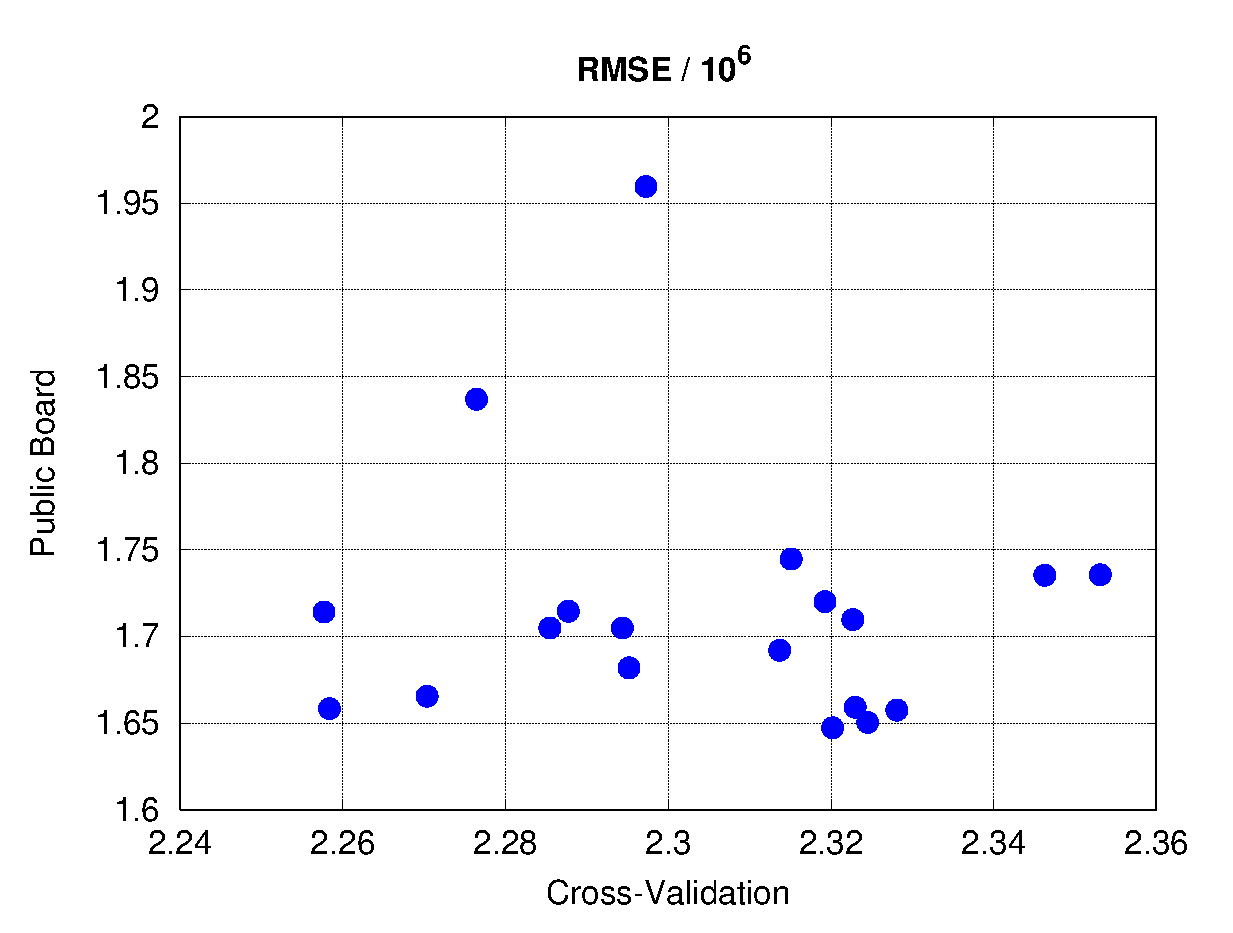
\includegraphics[width=5in]{figs/scores.eps} 
   \caption{RMSE of each submission.}
   \label{fig:cv_lb_error}
\end{figure}


\section{Conclusion}


\end{document}  